\chapter{जटिल बलगतिकी: शृंखलाएँ, एंज़ाइम और दोलन}\label{ch:b3:complex-kinetics}

विलोडित विलयन का एक बीकर रंगहीन हो जाता है, फिर अंबर, फिर नीला, फिर
पुनः रंगहीन, और कई मिनट तक ऐसा करता रहता है; एक तश्तरी में डालने पर
वही मिश्रण ऐसी सर्पिलें बनाता है जो घूमती और आगे बढ़ती हैं। जब बोरिस बेलौसोव ने
1951 में ऐसी अभिक्रिया का वर्णन किया, तो उनकी पांडुलिपि अस्वीकार कर दी गई: समीक्षक के
विचार में कोई रासायनिक निकाय आगे-पीछे नहीं चल सकता, क्योंकि उसे साम्य की ओर
ढलान पर ही उतरना चाहिए। वह ढलान पर उतरता ही है; बस सीधे नहीं उतरता।
यह अध्याय ऐसी अनेक-चरणीय क्रियाविधियों का अध्ययन करता है जिनके मध्यवर्ती
पुनर्जनित होते हैं: \omterm{def:b3:complex-kinetics:chain}{शृंखला अभिक्रियाएँ} और विस्फोट, वे अणु जिन्हें अकेले टूटने के लिए
संघट्टों की आवश्यकता होती है, \omterm{def:b3:complex-kinetics:enzyme}{एंज़ाइम}, और \omterm{def:b3:complex-kinetics:oscillating}{दोलनी अभिक्रियाएँ}, साथ ही
वे विधियाँ जो हाथ से मिलाने के लिए बहुत तीव्र अभिक्रियाओं का अनुसरण करती हैं।

\begin{recall}
प्रथम वर्ष के खंड ने अभिक्रिया क्रियाविधि को मूल चरणों के अनुक्रम के रूप में परिभाषित किया,
तथा दर-निर्धारक चरण, पूर्व-साम्य और स्थायी-अवस्था
सन्निकटन, और उत्प्रेरक परिभाषित किए। द्वितीय वर्ष के खंड ने मूलक
शृंखला के चरणों (आरंभन, संचरण, समापन), मूलक आरंभकों और
बहुलकीकरण की गतिक शृंखला लंबाई को नाम दिया, और न्यूनतम-वर्ग रेखाएँ समंजित कीं।
\Cref{ch:b3:rate-theories} ने \omterm{def:b3:rate-theories:tst}{संक्रमण-अवस्था सिद्धांत} और लगभग
\qty{e10}{L.mol^{-1}.s^{-1}} की विसरण सीमा दी।
\end{recall}

\section{शृंखला अभिक्रियाएँ}

\begin{definition}[शृंखला अभिक्रिया, शृंखला वाहक]\label{def:b3:complex-kinetics:chain}
\emph{शृंखला अभिक्रिया}\index{शृंखला अभिक्रिया} वह अभिक्रिया है जिसमें क्रियाशील
मध्यवर्ती, \emph{शृंखला वाहक}\index{शृंखला वाहक}, संचरण चरणों के एक चक्र द्वारा
पुनर्जनित होते हैं, जिससे आरंभन की एक घटना अनेक
अभिकारक अणुओं को रूपांतरित करती है।
\end{definition}

बोडेन्स्टाइन ने 1906 में $\ce{H2 + Br2 -> 2 HBr}$ की दर मापी और एक ऐसा नियम पाया जिसे
कोई अकेला चरण उत्पन्न नहीं कर सकता था: दर $[\ce{Br2}]^{1/2}$ के रूप में बढ़ती है और HBr
के संचय के साथ घटती है। क्रियाविधि 1919 में लिखी गई:
\begin{center}
\begin{tabular}{lll}
आरंभन & $\ce{Br2 -> 2 Br}$ & $k_1$ \\
संचरण & $\ce{Br + H2 -> HBr + H}$ & $k_2$ \\
संचरण & $\ce{H + Br2 -> HBr + Br}$ & $k_3$ \\
निरोधन & $\ce{H + HBr -> H2 + Br}$ & $k_4$ \\
समापन & $\ce{2 Br -> Br2}$ & $k_{-1}$
\end{tabular}
\end{center}
(किसी तीसरे पिंड M के साथ संघट्ट, जो आरंभन और समापन चरणों में ऊर्जा
लाते और ले जाते हैं, अंतर्निहित छोड़ दिए गए हैं)।

\begin{theorem}[हाइड्रोजन--ब्रोमीन दर नियम]\label{thm:b3:complex-kinetics:hbr}
Br और H के लिए स्थायी-अवस्था सन्निकटन के साथ क्रियाविधि की दर
$v = \frac12\,\dd[\ce{HBr}]/\dd t$ यह है:
\[
  v = \frac{k[\ce{H2}][\ce{Br2}]^{1/2}}{1 + k'[\ce{HBr}]/[\ce{Br2}]},
  \qquad k = k_2\Bigl(\frac{k_1}{k_{-1}}\Bigr)^{1/2},\ k' = \frac{k_4}{k_3}.
\]
\end{theorem}

\begin{proof}
H के लिए स्थायी अवस्था: $k_2[\ce{Br}][\ce{H2}] = k_3[\ce{H}][\ce{Br2}] + k_4[\ce{H}][\ce{HBr}]$। Br के लिए स्थायी अवस्था:
$2k_1[\ce{Br2}] - k_2[\ce{Br}][\ce{H2}] + k_3[\ce{H}][\ce{Br2}] + k_4[\ce{H}][\ce{HBr}] - 2k_{-1}[\ce{Br}]^2 = 0$। दोनों
समीकरणों को जोड़ने पर संचरण पद निरस्त हो जाते हैं: $k_1[\ce{Br2}] = k_{-1}[\ce{Br}]^2$, अतः $[\ce{Br}] =
(k_1/k_{-1})^{1/2}[\ce{Br2}]^{1/2}$। तब $[\ce{H}] = k_2[\ce{Br}][\ce{H2}]/(k_3[\ce{Br2}] + k_4[\ce{HBr}])$ और
\[
  \frac{\dd[\ce{HBr}]}{\dd t} = k_2[\ce{Br}][\ce{H2}] + k_3[\ce{H}][\ce{Br2}] - k_4[\ce{H}][\ce{HBr}] = 2k_3[\ce{H}][\ce{Br2}]
  = \frac{2k_2[\ce{Br}][\ce{H2}]}{1 + (k_4/k_3)[\ce{HBr}]/[\ce{Br2}]},
\]
पहले समीकरण का उपयोग करके; $[\ce{Br}]$ प्रतिस्थापित करने पर परिणाम मिलता है।
\end{proof}

\begin{omfigure}
\begin{tikzpicture}[font=\small, >=Stealth]
  \node[draw, circle, minimum size=9mm, omDef, thick] (br) at (0,0) {Br};
  \node[draw, circle, minimum size=9mm, omThm, thick] (h) at (4,0) {H};
  \draw[->, thick] (br) to[bend left=35] node[midway, above, align=center] {$+\,\ce{H2}$\\ $\to$ HBr} (h);
  \draw[->, thick] (h) to[bend left=35] node[midway, below, align=center] {$+\,\ce{Br2}$\\ $\to$ HBr} (br);
  \draw[->, thick, black!60] (-2.4,0) -- (br) node[pos=0, left, align=right] {आरंभन\\ $\ce{Br2 -> 2 Br}$};
  \draw[->, thick, black!60] (br) -- (0,-2.0) node[below, align=center] {समापन\\ $\ce{2 Br -> Br2}$};
  \draw[->, thick, black!60, dashed] (h) -- (6.2,-1.2) node[below, align=center] {निरोधन\\ $\ce{H + HBr -> H2 + Br}$};
\end{tikzpicture}

{\small हाइड्रोजन--ब्रोमीन शृंखला का संचरण चक्र: हर चक्कर एक \ce{H2} और एक \ce{Br2}
खपाता है, दो HBr बनाता है और वह ब्रोमीन परमाणु लौटा देता है जिसने उसे
आरंभ किया था। आरंभन चक्र को वाहकों की आपूर्ति करता है, समापन उन्हें हटाता है;
निरोधन चरण एक H परमाणु को, पहले से बने एक HBr की कीमत पर,
वापस Br में बदल देता है।}
\end{omfigure}

\begin{omfigure}
\begin{tikzpicture}
\begin{axis}[name=ca, width=0.47\linewidth, height=5.2cm, xmin=0, xmax=800, ymin=0, ymax=1,
  axis lines=left, xlabel={$t$ (समानीत)}, ylabel={$[\ce{HBr}]/2[\ce{H2}]_0$},
  tick label style={font=\small}, label style={font=\small}]
\addplot[omDef, thick] table[x=t, y expr=\thisrow{HBr}/2] {figdata/out/bachelor-3-chain-kinetics.dat};
\end{axis}
\begin{axis}[at={(ca.east)}, anchor=west, xshift=1.4cm, width=0.47\linewidth, height=5.2cm,
  xmin=0, xmax=60, ymin=0, ymax=2.2, axis lines=left, xlabel={$t$ (समानीत)},
  ylabel={दर $\times 10^3$}, tick label style={font=\small}, label style={font=\small},
  legend style={font=\scriptsize, draw=none, at={(0.97,0.03)}, anchor=south east},
  legend cell align=left]
\addplot[omDef, thick] table[x=t, y expr=1000*\thisrow{v}] {figdata/out/bachelor-3-chain-kinetics.dat};
\addplot[omThm, thick, dashed] table[x=t, y expr=1000*\thisrow{vss}] {figdata/out/bachelor-3-chain-kinetics.dat};
\legend{पूर्ण क्रियाविधि, स्थायी-अवस्था नियम}
\end{axis}
\end{tikzpicture}

{\small चरण-दर-चरण समाकलित हाइड्रोजन--ब्रोमीन क्रियाविधि (मॉडल दर
स्थिरांक, समानीत इकाइयाँ, $k' = 0.1$): समय के विरुद्ध रूपांतरण (बाएँ), और
पूर्ण क्रियाविधि की दर $\frac12\dd[\ce{HBr}]/\dd t$ की स्थायी-अवस्था नियम से तुलना (दाएँ)।
एक प्रेरण काल के बाद, जिसके दौरान ब्रोमीन परमाणु संचित होते हैं, दोनों
1\,\% से बेहतर मेल खाते हैं।}
\end{omfigure}

\begin{method}[शृंखला क्रियाविधि का दर नियम]\label{met:b3:complex-kinetics:steady-state-chain}
\begin{enumerate}
  \item हर \omterm{def:b3:complex-kinetics:chain}{शृंखला वाहक} के लिए एक स्थायी-अवस्था समीकरण लिखिए।
  \item उन्हें जोड़िए: संचरण चरण, जो केवल एक वाहक को दूसरे से बदलते हैं,
        निरस्त हो जाते हैं, और आरंभन समापन के बराबर रह जाता है; इससे
        वाहक सांद्रता मिलती है।
  \item एक वाहक के समीकरण से अन्य वाहकों को व्यक्त कीजिए।
  \item संचरण चरणों से किसी उत्पाद के निर्माण की दर लिखिए।
\end{enumerate}
\end{method}

आरंभन की प्रति घटना संचरण चक्रों की संख्या, यहाँ $v/k_1[\ce{Br2}]$,
द्वितीय वर्ष के खंड की गतिक शृंखला लंबाई है; हाइड्रोजन--ब्रोमीन अभिक्रिया के लिए
यह परिस्थितियों के अनुसार $10^3$ से $10^6$ की कोटि की है। उत्पाद द्वारा निरोधन
समझाता है कि दर अभिकारकों के खपने की तुलना में तेज़ी से क्यों गिरती है।

\section{शाखित शृंखलाएँ और विस्फोट}

\begin{definition}[शृंखला शाखन, विस्फोट सीमाएँ]\label{def:b3:complex-kinetics:branching}
\emph{शृंखला शाखन}\index{शृंखला शाखन} ऐसा संचरण चरण है जो जितने
\omterm{def:b3:complex-kinetics:chain}{शृंखला वाहक} खपाता है उससे अधिक उत्पन्न करता है, जैसे $\ce{H + O2 -> OH + O}$, जो एक
वाहक को दो में बदल देता है। किसी मिश्रण की \emph{विस्फोट सीमाएँ}\index{विस्फोट सीमाएँ}
दिए हुए ताप पर वे दाब हैं जिन पर उसकी मंद अभिक्रिया
विस्फोट में बदल जाती है।
\end{definition}

\begin{proposition}[शाखन निकष]\label{prop:b3:complex-kinetics:branching}
मान लीजिए वाहक दर $v_i$ पर बनते हैं, दर
स्थिरांक $f$ के साथ शाखन से गुणित होते हैं और दर स्थिरांक $g$ के साथ समापन से लुप्त होते हैं:
$\dd n/\dd t = v_i + (f - g)n$। यदि $f < g$, तो $n$ स्थायी मान $v_i/(g - f)$ की ओर प्रवृत्त होता है; यदि
$f > g$, तो $n$ चरघातांकी रूप से बढ़ता है और अभिक्रिया विस्फोटित होती है।
\end{proposition}

\begin{proof}
रैखिक समीकरण का हल $n(t) = \frac{v_i}{g - f}\bigl(1 - \eu^{-(g - f)t}\bigr)$ है, जो
$v_i/(g - f)$ की ओर प्रवृत्त होता है जब $g > f$; जब $f > g$, तो घातांक धनात्मक है और $n$
असीमित रूप से $\eu^{(f - g)t}$ की तरह बढ़ता है (जब तक अभिकारक समाप्त न हो जाएँ)।
\end{proof}

कुछ सौ अंश पर हाइड्रोजन--ऑक्सीजन मिश्रणों के लिए $f$ दाब के साथ बढ़ता है
(यह $[\ce{O2}]$ के समानुपाती है), पात्र की दीवारों पर समापन
निम्न दाब पर तीव्र होता है (मूलक आसानी से वहाँ विसरित हो जाते हैं), और
त्रि-पिंड संघट्टों ($\ce{H + O2 + M -> HO2 + M}$) द्वारा समापन दाब के वर्ग के रूप में
बढ़ता है। शाखन एक पहली सीमा, जो दीवारें निर्धारित करती हैं, और एक
दूसरी सीमा, जो त्रि-पिंड समापन निर्धारित करता है, के बीच जीतता है; और ऊँचे दाब पर एक तीसरी
सीमा प्रकट होती है जहाँ मुक्त ऊष्मा अब बाहर नहीं निकल पाती। अंतिम
तापीय विस्फोट है, जो शाखन के बजाय ताप के साथ दर की चरघातांकी वृद्धि से
प्रेरित होता है; अधिकांश औद्योगिक विस्फोट इसी
प्रकार के होते हैं।

\section{एकाण्विक अभिक्रियाएँ}

साइक्लोप्रोपेन जैसा अणु अकेले समावयवित होता है, सामान्य दाबों पर प्रथम-कोटि
बलगतिकी के साथ; फिर भी निम्न दाब पर दर स्थिरांक गिर जाता है। आवश्यक
ऊर्जा संघट्टों से आती है।

\begin{definition}[लिंडेमान क्रियाविधि, पतन क्षेत्र]\label{def:b3:complex-kinetics:lindemann}
किसी एकाण्विक अभिक्रिया की \emph{लिंडेमान क्रियाविधि}\index{लिंडेमान क्रियाविधि}
अनुक्रम $\mathrm{A + M \rightleftharpoons A^* + M}$ ($k_1$, $k_{-1}$) है, अर्थात् किसी भी अणु M के साथ संघट्ट द्वारा
सक्रियण और निष्क्रियण, जिसके बाद $\mathrm{A^* \to P}$ ($k_2$)।
\emph{पतन क्षेत्र}\index{पतन क्षेत्र} दाबों का वह परास है जहाँ
प्रेक्षित प्रथम-कोटि दर स्थिरांक अपने उच्च-दाब मान से
द्वितीय-कोटि व्यवहार की ओर गिरता है।
\end{definition}

\begin{theorem}[लिंडेमान दर स्थिरांक]\label{thm:b3:complex-kinetics:lindemann}
$\mathrm{A^*}$ के लिए स्थायी-अवस्था सन्निकटन के साथ $v = k_{\mathrm{uni}}[\mathrm A]$, जहाँ
\[
  k_{\mathrm{uni}} = \frac{k_1k_2[\mathrm M]}{k_{-1}[\mathrm M] + k_2},
\]
जो उच्च दाब पर $k_\infty = k_1k_2/k_{-1}$ की ओर (प्रथम कोटि) और निम्न दाब पर $k_1[\mathrm M]$ की ओर
(द्वितीय कोटि) प्रवृत्त होता है; यह $k_\infty/2$ है, $[\mathrm M]_{1/2} = k_2/k_{-1}$ पर।
\end{theorem}

\begin{proof}
$\dd[\mathrm{A^*}]/\dd t = k_1[\mathrm A][\mathrm M] - k_{-1}[\mathrm{A^*}][\mathrm M] - k_2[\mathrm{A^*}] = 0$ से $[\mathrm{A^*}] =
k_1[\mathrm A][\mathrm M]/(k_{-1}[\mathrm M] + k_2)$ और $v = k_2[\mathrm{A^*}]$। यदि $k_{-1}[\mathrm M] \gg k_2$, तो निष्क्रियण
अभिक्रिया से आगे निकल जाता है और $\mathrm{A^*}$ पूर्व-साम्य में है: $k_{\mathrm{uni}} \to k_1k_2/k_{-1}$। यदि $k_{-1}[\mathrm M]
\ll k_2$, तो हर सक्रियित अणु अभिक्रिया करता है और सक्रियण दर-निर्धारक है:
$k_{\mathrm{uni}} \to k_1[\mathrm M]$।
\end{proof}

\begin{omfigure}
\begin{tikzpicture}
\begin{axis}[width=0.66\linewidth, height=5.4cm, xmode=log, ymode=log, xmin=1e-10, xmax=1e-2,
  ymin=1e-8, ymax=4e-3, axis lines=left, xlabel={$[\mathrm M]$ / \unit{mol.L^{-1}}},
  ylabel={$k_{\mathrm{uni}}$ / \unit{s^{-1}}}, tick label style={font=\small}, label style={font=\small}]
\addplot[black!40, dashed] table[x=M, y=low] {figdata/out/bachelor-3-lindemann.dat};
\addplot[black!40, dashed] table[x=M, y=high] {figdata/out/bachelor-3-lindemann.dat};
\addplot[omDef, very thick] table[x=M, y=k] {figdata/out/bachelor-3-lindemann.dat};
\node[font=\scriptsize, anchor=south, rotate=39] at (axis cs:4e-9,2.5e-5) {$k_1[\mathrm M]$};
\node[font=\scriptsize, anchor=south] at (axis cs:3e-4,1e-3) {$k_\infty$};
\draw[black!50, densely dotted] (axis cs:1e-6,1e-8) -- (axis cs:1e-6,5e-4);
\node[font=\scriptsize, anchor=north west] at (axis cs:1.2e-6,2e-7) {$[\mathrm M]_{1/2}$};
\end{axis}
\end{tikzpicture}

{\small लिंडेमान पतन वक्र (मॉडल स्थिरांक): उच्च दाब पर सीमांत स्थिरांक $k_\infty$ के साथ
प्रथम कोटि, निम्न दाब पर द्वितीय कोटि ($k_1[\mathrm M]$),
और $k_\infty$ का आधा, $[\mathrm M]_{1/2} = k_2/k_{-1}$ पर। वास्तविक पतन वक्र अधिक चौड़े होते हैं: ऊर्जित अणु का दर
स्थिरांक $k_2$ उसकी ऊर्जा के साथ बढ़ता है।}
\end{omfigure}

\section{एंज़ाइम बलगतिकी}

\begin{definition}[एंज़ाइम, सक्रिय स्थल, एंज़ाइम--क्रियाधार संकुल]\label{def:b3:complex-kinetics:enzyme}
\emph{एंज़ाइम}\index{एंज़ाइम} एक जैविक उत्प्रेरक है, लगभग सदा एक प्रोटीन,
जो अपने क्रियाधार की किसी विशिष्ट अभिक्रिया को तीव्र करता है। \emph{सक्रिय
स्थल}\index{सक्रिय स्थल} एंज़ाइम की वह गुहिका है जहाँ क्रियाधार बँधता है
और अभिक्रिया करता है; बँधी हुई स्पीशीज़ \emph{एंज़ाइम--क्रियाधार
संकुल}\index{एंज़ाइम--क्रियाधार संकुल} ES है।
\end{definition}

\begin{definition}[माइकेलिस स्थिरांक, अधिकतम दर, उत्प्रेरकी और विशिष्टता स्थिरांक]\label{def:b3:complex-kinetics:michaelis}
क्रियाविधि $\mathrm{E + S \rightleftharpoons ES \to E + P}$ ($k_1$, $k_{-1}$, $k_2$) के लिए, कुल \omterm{def:b3:complex-kinetics:enzyme}{एंज़ाइम} सांद्रता $[\mathrm E]_0$ पर,
\emph{उत्प्रेरकी स्थिरांक}\index{उत्प्रेरकी स्थिरांक} $k_{\mathrm{cat}} = k_2$ है,
\emph{अधिकतम दर}\index{अधिकतम दर} $V_{\max} = k_{\mathrm{cat}}[\mathrm E]_0$, \emph{माइकेलिस स्थिरांक}
\index{माइकेलिस स्थिरांक} $K_M = (k_{-1} + k_2)/k_1$, और \emph{विशिष्टता स्थिरांक}
\index{विशिष्टता स्थिरांक} $k_{\mathrm{cat}}/K_M$।
\end{definition}

\begin{theorem}[माइकेलिस--मेंटेन समीकरण]\label{thm:b3:complex-kinetics:michaelis-menten}
जब $[\mathrm S] \gg [\mathrm E]_0$ और ES स्थायी अवस्था में हो, तो उत्पाद के निर्माण की
प्रारंभिक दर यह है:
\[
  v = \frac{V_{\max}[\mathrm S]}{K_M + [\mathrm S]} .
\]
यह कथन \emph{माइकेलिस--मेंटेन समीकरण}\index{माइकेलिस--मेंटेन समीकरण} है।
\end{theorem}

\begin{proof}
स्थायी अवस्था: $k_1[\mathrm E][\mathrm S] = (k_{-1} + k_2)[\mathrm{ES}]$, और $[\mathrm E] = [\mathrm E]_0 - [\mathrm{ES}]$ (मुक्त
क्रियाधार व्यावहारिक रूप से पूरा क्रियाधार है, क्योंकि $[\mathrm S] \gg [\mathrm E]_0$)। अतः $[\mathrm{ES}]
= [\mathrm E]_0[\mathrm S]/(K_M + [\mathrm S])$ और $v = k_2[\mathrm{ES}]$।
\end{proof}

\begin{remark}
माइकेलिस और मेंटेन (1913) ने इसके स्थान पर E, S और
ES का तीव्र पूर्व-साम्य माना था; वही समीकरण निकलता है, जिसमें $K_M$ के स्थान पर वियोजन स्थिरांक
$k_{-1}/k_1$ होता है, जो $K_M$ की सीमा है, जब $k_2 \ll k_{-1}$। \omterm{def:b3:complex-kinetics:michaelis}{उत्प्रेरकी स्थिरांक} वह है
जिसे जैवरसायनज्ञ \omterm{def:b3:complex-kinetics:enzyme}{एंज़ाइम} की आवर्त संख्या कहते हैं: क्रियाधार
अणुओं की वह संख्या जिसे एक \omterm{def:b3:complex-kinetics:enzyme}{सक्रिय स्थल} संतृप्त होने पर प्रति सेकंड रूपांतरित करता है।
\end{remark}

$[\mathrm S] = K_M$ पर दर $V_{\max}/2$ है; $[\mathrm S] \ll K_M$ पर यह $(k_{\mathrm{cat}}/K_M)[\mathrm E]_0[\mathrm S]$ है:
\omterm{def:b3:complex-kinetics:michaelis}{विशिष्टता स्थिरांक} मुक्त \omterm{def:b3:complex-kinetics:enzyme}{एंज़ाइम} का अपने क्रियाधार के साथ द्वितीय-कोटि दर स्थिरांक है,
और यह उस दर से अधिक नहीं हो सकता जिस पर वे मिलते हैं, यानी
\cref{ch:b3:rate-theories} की विसरण सीमा। कुछ \omterm{def:b3:complex-kinetics:enzyme}{एंज़ाइम} उसके निकट आते हैं;
कई हज़ार \omterm{def:b3:complex-kinetics:enzyme}{एंज़ाइमों} के एक सर्वेक्षण में ``औसत'' \omterm{def:b3:complex-kinetics:enzyme}{एंज़ाइम} का $k_{\mathrm{cat}}/K_M$ लगभग
$10^5$~\unit{L.mol^{-1}.s^{-1}} है, कोई चार परिमाण-कोटि नीचे।

\begin{proposition}[लाइनवीवर--बर्क रूप]\label{prop:b3:complex-kinetics:lineweaver}
\omterm{thm:b3:complex-kinetics:michaelis-menten}{माइकेलिस--मेंटेन समीकरण} इसके तुल्य है:
\[
  \frac1v = \frac{1}{V_{\max}} + \frac{K_M}{V_{\max}}\,\frac{1}{[\mathrm S]},
\]
जो $1/v$ की $1/[\mathrm S]$ के विरुद्ध एक सीधी रेखा है, अंतःखंड $1/V_{\max}$, ढलान $K_M/V_{\max}$, और
अंतःखंड $-1/K_M$ के साथ, $1/[\mathrm S]$ अक्ष पर।
\end{proposition}

\begin{proof}
व्युत्क्रम लीजिए: $1/v = (K_M + [\mathrm S])/(V_{\max}[\mathrm S])$। $1/v = 0$ पर $1/[\mathrm S] = -1/K_M$।
\end{proof}

\begin{method}[अरैखिक न्यूनतम वर्ग से $K_M$ और $V_{\max}$]\label{met:b3:complex-kinetics:mm-fit}
\begin{enumerate}
  \item लगभग $K_M/5$ से $10K_M$ तक फैली क्रियाधार सांद्रताओं पर
        प्रारंभिक दरें मापिए।
  \item $v = V_{\max}[\mathrm S]/(K_M + [\mathrm S])$ को सीधे समंजित कीजिए, $\sum(v_i - v(\mathrm S_i))^2$ को न्यूनतम करके (पुनरावर्ती रूप से,
        लाइनवीवर--बर्क रेखा के मानों से आरंभ करते हुए); मानक
        त्रुटियाँ अवशिष्टों से और हर प्राचल के प्रति $v$ की
        संवेदनशीलता से आती हैं।
  \item लाइनवीवर--बर्क आलेख का उपयोग केवल पैटर्न देखने के लिए कीजिए: छोटी
        दरों का व्युत्क्रम उनकी त्रुटियों को बढ़ा देता है, अतः $1/v$ से होकर न्यूनतम-वर्ग रेखा
        पर सबसे कम परिशुद्ध बिंदुओं का प्रभुत्व होता है, और उसके प्राचल
        अभिनत होते हैं।
\end{enumerate}
\end{method}

\begin{definition}[संदमन]\label{def:b3:complex-kinetics:inhibition}
एक संदमक I \omterm{def:b3:complex-kinetics:enzyme}{एंज़ाइम} से उत्क्रमणीय रूप से बँधता है। \emph{स्पर्धी
संदमन}\index{स्पर्धी संदमन} में वह केवल मुक्त \omterm{def:b3:complex-kinetics:enzyme}{एंज़ाइम} से, \omterm{def:b3:complex-kinetics:enzyme}{सक्रिय
स्थल} पर, बँधता है, \emph{संदमन स्थिरांक}\index{संदमन स्थिरांक} $K_i$ के साथ
(EI का वियोजन स्थिरांक); \emph{अस्पर्धी संदमन}\index{अस्पर्धी संदमन}
में वह केवल ES से बँधता है, स्थिरांक $K_i'$ के साथ; \emph{मिश्र
संदमन}\index{मिश्र संदमन} में वह दोनों से बँधता है।
\end{definition}

\begin{proposition}[संदमित दर नियम]\label{prop:b3:complex-kinetics:inhibition-laws}
$\alpha = 1 + [\mathrm I]/K_i$ और $\alpha' = 1 + [\mathrm I]/K_i'$ के साथ दर
माइकेलिस--मेंटेन रूप $v = V^{\mathrm{app}}[\mathrm S]/(K_M^{\mathrm{app}} + [\mathrm S])$ बनाए रखती है, जहाँ: स्पर्धी,
$K_M^{\mathrm{app}} = \alpha K_M$, $V^{\mathrm{app}} = V_{\max}$; अस्पर्धी, $K_M^{\mathrm{app}} = K_M/\alpha'$, $V^{\mathrm{app}} =
V_{\max}/\alpha'$; मिश्र, $K_M^{\mathrm{app}} = \alpha K_M/\alpha'$, $V^{\mathrm{app}} = V_{\max}/\alpha'$।
\end{proposition}

\begin{proof}
मिश्र स्थिति (बाकी इसकी सीमाएँ $K_i' \to \infty$ और $K_i \to \infty$ हैं): \omterm{def:b3:complex-kinetics:enzyme}{एंज़ाइम}
E, EI, ES और ESI में बँटा है, जहाँ $[\mathrm{EI}] = [\mathrm E][\mathrm I]/K_i$, $[\mathrm{ESI}] = [\mathrm{ES}][\mathrm I]/K_i'$
और स्थायी अवस्था $[\mathrm E][\mathrm S] = K_M[\mathrm{ES}]$। अतः $[\mathrm E]_0 = [\mathrm E]\alpha + [\mathrm{ES}]\alpha' =
[\mathrm{ES}](\alpha K_M/[\mathrm S] + \alpha')$ और $v = k_2[\mathrm{ES}] = V_{\max}[\mathrm S]/(\alpha K_M + \alpha'[\mathrm S])$; अंश
और हर को $\alpha'$ से भाग देने पर बताया गया रूप मिलता है।
\end{proof}

\begin{method}[संदमन के प्रकार की पहचान]\label{met:b3:complex-kinetics:inhibition-type}
\begin{enumerate}
  \item अनेक संदमक सांद्रताओं पर $v([\mathrm S])$ मापिए और
        लाइनवीवर--बर्क रेखाएँ खींचिए।
  \item $1/v$ अक्ष पर मिलने वाली रेखाएँ (समान $V_{\max}$): स्पर्धी; क्रियाधार की बड़ी अधिकता
        संदमक पर विजय पा लेती है।
  \item समांतर रेखाएँ (ढलान $K_M/V_{\max}$ अपरिवर्तित): अस्पर्धी।
  \item $1/v$ अक्ष के बाईं ओर मिलने वाली रेखाएँ: मिश्र।
  \item $K_i$ प्राप्त कीजिए, आभासी स्थिरांकों को $[\mathrm I]$ के विरुद्ध समंजित करके:
        स्पर्धी संदमक के लिए $K_M^{\mathrm{app}} = K_M + (K_M/K_i)[\mathrm I]$, एक सीधी रेखा।
\end{enumerate}
\end{method}

\begin{omfigure}
\begin{tikzpicture}
\begin{axis}[name=mv, width=0.47\linewidth, height=5.4cm, xmin=0, xmax=8, ymin=0, ymax=0.55,
  axis lines=left, xlabel={$[\mathrm S]$ / mM}, ylabel={$v$ / \unit{\micro M.s^{-1}}},
  tick label style={font=\small}, label style={font=\small},
  legend style={font=\scriptsize, draw=none, fill=white, fill opacity=0.85, text opacity=1,
  at={(0.97,0.03)}, anchor=south east}, legend cell align=left]
\addplot[black, thick] table[x=S, y=none] {figdata/out/bachelor-3-michaelis-menten-model.dat};
\addplot[omDef, thick] table[x=S, y=comp] {figdata/out/bachelor-3-michaelis-menten-model.dat};
\addplot[omThm, thick] table[x=S, y=uncomp] {figdata/out/bachelor-3-michaelis-menten-model.dat};
\draw[black!40, densely dotted] (axis cs:0,0.25) -- (axis cs:0.8,0.25) -- (axis cs:0.8,0);
\node[font=\scriptsize, anchor=north west] at (axis cs:0.85,0.12) {$K_M$};
\legend{संदमक नहीं, स्पर्धी, अस्पर्धी}
\end{axis}
\begin{axis}[at={(mv.east)}, anchor=west, xshift=1.5cm, width=0.47\linewidth, height=5.4cm,
  xmin=-2.5, xmax=3.5, ymin=0, ymax=12, axis x line=middle, axis y line=middle,
  tick label style={font=\small}, xtick={-2,-1,1,2,3}]
\node[font=\small, anchor=south east] at (axis cs:3.5,0.3) {$1/[\mathrm S]$};
\node[font=\small, anchor=north west] at (axis cs:0.12,12) {$1/v$};
\addplot[black, thick, domain=-1.25:3.5] {1.6*x + 2};
\addplot[omDef, thick, domain=-0.4167:3.5] {4.8*x + 2};
\addplot[omThm, thick, domain=-2.5:3.5] {1.6*x + 4};
\end{axis}
\end{tikzpicture}

{\small $K_M = \qty{0.80}{mM}$ और $V_{\max} = \qty{0.50}{\micro M.s^{-1}}$ के साथ माइकेलिस--मेंटेन बलगतिकी
(मॉडल): संदमक नहीं (काला), $[\mathrm I] = 2K_i$ पर एक स्पर्धी संदमक (नीला,
$K_M$ तिगुना, $V_{\max}$ वही) और $[\mathrm I] = K_i'$ पर एक अस्पर्धी संदमक (लाल, $K_M$ और
$V_{\max}$ आधे)। दाएँ: लाइनवीवर--बर्क रेखाएँ; स्पर्धी रेखा
असंदमित रेखा से $1/v$ अक्ष पर मिलती है, अस्पर्धी रेखा उसके समांतर है
($1/[\mathrm S]$, \unit{mM^{-1}} में, $1/v$, \unit{s.\micro M^{-1}} में)।}
\end{omfigure}

\section{स्वउत्प्रेरण, दोलन और तीव्र अभिक्रियाएँ}

\begin{definition}[स्वउत्प्रेरकी अभिक्रिया]\label{def:b3:complex-kinetics:autocatalysis}
\emph{स्वउत्प्रेरकी अभिक्रिया}\index{स्वउत्प्रेरकी अभिक्रिया} वह है जिसमें कोई
उत्पाद अपने ही निर्माण को उत्प्रेरित करता है, जैसे $\mathrm{A + X \to 2\,X}$ में।
\end{definition}

\begin{proposition}[लॉजिस्टिक नियम]\label{prop:b3:complex-kinetics:logistic}
$\mathrm{A + X \to 2\,X}$ के लिए, दर स्थिरांक $k$ और प्रारंभिक सांद्रताओं $a_0$ और $x_0$ के साथ,
$N = a_0 + x_0$ लेकर,
\[
  x(t) = \frac{N}{1 + (N/x_0 - 1)\eu^{-kNt}},
\]
एक S-आकार का वक्र, जो $t_{1/2} = \ln(N/x_0 - 1)/kN$ पर अपने अंतिम मान के आधे तक पहुँचता है।
\end{proposition}

\begin{proof}
$\dd x/\dd t = kx(N - x)$, क्योंकि $a = N - x$। चरों को पृथक करने पर $\frac{\dd x}{x(N - x)} = \frac1N\bigl(\frac1x + \frac{1}{N - x}\bigr)\dd x
= k\,\dd t$, अतः $\ln\frac{x}{N - x} = kNt + \ln\frac{x_0}{N - x_0}$, जो पुनर्व्यवस्थित होकर बताया गया रूप देता है;
$x = N/2$ जब $(N/x_0 - 1)\eu^{-kNt} = 1$।
\end{proof}

\begin{definition}[दोलनी अभिक्रिया, सीमा चक्र]\label{def:b3:complex-kinetics:oscillating}
\emph{दोलनी अभिक्रिया}\index{दोलनी अभिक्रिया} वह है जिसमें
मध्यवर्तियों की सांद्रताएँ आवर्ती रूप से बढ़ती और घटती हैं जबकि समग्र
अभिक्रिया साम्य की ओर बढ़ती है। \emph{सीमा चक्र}\index{सीमा चक्र}
सांद्रताओं के आकाश में एक संवृत प्रक्षेप-पथ है जिसकी ओर पड़ोसी
प्रक्षेप-पथ अभिसरित होते हैं, ताकि दोलन का आयाम
आरंभ-बिंदु से स्वतंत्र हो।
\end{definition}

\begin{theorem}[लोत्का--वोल्टेरा मॉडल]\label{thm:b3:complex-kinetics:lotka-volterra}
स्वउत्प्रेरकी योजना $\mathrm{A + X \to 2\,X}$, $\mathrm{X + Y \to 2\,Y}$, $\mathrm{Y \to B}$ के लिए, A को
स्थिर रखते हुए, सांद्रताएँ $\dot x = x(a - by)$, $\dot y = y(dx - c)$ का पालन करती हैं, धनात्मक
स्थिरांकों के साथ, और राशि
\[
  V = dx - c\ln x + by - a\ln y
\]
हर प्रक्षेप-पथ के अनुदिश अचर है: प्रक्षेप-पथ स्थायी अवस्था $(c/d, a/b)$ के
चारों ओर संवृत वक्र हैं, और सांद्रताएँ ऐसे
आयाम से दोलन करती हैं जो आरंभ-बिंदु द्वारा निर्धारित है।
\end{theorem}

\begin{proof}
$\dot V = (d - c/x)\dot x + (b - a/y)\dot y = (dx - c)(a - by) + (by - a)(dx - c) = 0$। $V$, $(c/d, a/b)$ पर
एकमात्र निम्निष्ठ वाले दो उत्तल फलनों का योग है, अतः उसके समस्तर
वक्र उस बिंदु के चारों ओर संवृत वक्र हैं; प्रक्षेप-पथ उनमें से एक पर बना रहता है
और, क्योंकि वेग अन्यत्र कभी लुप्त नहीं होता, उसका आवर्ती रूप से चक्कर लगाता है।
\end{proof}

लोत्का--वोल्टेरा दोलन भंगुर हैं: हर आरंभ-बिंदु अपनी
कक्षा देता है, और कोई भी विक्षोभ निकाय को दूसरी कक्षा पर ले जाता है। वास्तविक रासायनिक
दोलित्रों का एक \omterm{def:b3:complex-kinetics:oscillating}{सीमा चक्र} होता है, जिसके लिए ऐसी अरैखिकता चाहिए जो
स्थायी अवस्था को अस्थिर करे।

\begin{proposition}[ब्रसेलेटर की अस्थिरता]\label{prop:b3:complex-kinetics:hopf}
मॉडल $\dot X = A - (B + 1)X + X^2Y$, $\dot Y = BX - X^2Y$ (समानीत सांद्रताएँ,
$A$ और $B$ स्थिर) की एकमात्र स्थायी अवस्था $(A, B/A)$ है, जो
स्थिर है यदि $B < 1 + A^2$ और अस्थिर यदि $B > 1 + A^2$; तब निकाय एक
\omterm{def:b3:complex-kinetics:oscillating}{सीमा चक्र} पर स्थिर हो जाता है।
\end{proposition}

\begin{proof}
दोनों अवकलजों को शून्य रखने पर: $BX = X^2Y$ से $XY = B$, और फिर $A - X = 0$।
$(A, B/A)$ पर जैकोबी आव्यूह यह है:
\[
  \begin{pmatrix} -(B + 1) + 2XY & X^2 \\ B - 2XY & -X^2 \end{pmatrix}
  = \begin{pmatrix} B - 1 & A^2 \\ -B & -A^2 \end{pmatrix},
\]
जिसका अनुरेख $B - 1 - A^2$ और सारणिक $A^2 > 0$ है। छोटे विचलन
$\eu^{\lambda t}$ के रूप में विकसित होते हैं, जहाँ $\lambda$ \omterm{def:b3:quantum-model-systems:operator}{अभिलक्षणिक मान} हैं, जिनका गुणनफल सारणिक (धनात्मक)
और योग अनुरेख है: दोनों के वास्तविक भाग ऋणात्मक हैं जब अनुरेख
ऋणात्मक हो, धनात्मक जब वह धनात्मक हो। $B > 1 + A^2$ के लिए \omterm{def:b3:complex-kinetics:oscillating}{सीमा
चक्र} का अस्तित्व (प्रक्षेप-पथ एक परिबद्ध क्षेत्र में सीमित रहते हैं)
स्वीकार किया गया है।
\end{proof}

\begin{method}[किसी स्थायी अवस्था की रैखिक स्थिरता]\label{met:b3:complex-kinetics:stability}
\begin{enumerate}
  \item सभी काल-अवकलजों को शून्य रखकर स्थायी अवस्था ज्ञात कीजिए।
  \item वहाँ दरों के आंशिक अवकलजों का जैकोबी आव्यूह परिकलित कीजिए।
  \item दो चरों के लिए: स्थिर, यदि अनुरेख ऋणात्मक और सारणिक
        धनात्मक हो; सम्मिश्र \omterm{def:b3:quantum-model-systems:operator}{अभिलक्षणिक मानों} वाली अस्थिर अवस्था
        ($\mathrm{tr}^2 < 4\det$) बढ़ते दोलन देती है, एक संभावित \omterm{def:b3:complex-kinetics:oscillating}{सीमा चक्र}।
\end{enumerate}
\end{method}

\begin{omfigure}
\begin{tikzpicture}
\begin{axis}[name=bs, width=0.62\linewidth, height=4.6cm, xmin=0, xmax=40, ymin=0, ymax=5.2,
  axis lines=left, xlabel={$t$ (समानीत)}, ylabel={सांद्रता},
  tick label style={font=\small}, label style={font=\small},
  legend style={font=\scriptsize, draw=none, at={(1.03,0.98)}, anchor=north west}]
\addplot[omDef, thick] table[x=t, y=X] {figdata/out/bachelor-3-oscillations-series.dat};
\addplot[omThm, thick] table[x=t, y=Y] {figdata/out/bachelor-3-oscillations-series.dat};
\legend{$X$, $Y$}
\end{axis}
\begin{axis}[name=ph, at={(bs.below south west)}, anchor=north west, yshift=-0.6cm,
  width=0.42\linewidth, height=5.0cm, xmin=0, xmax=4.8, ymin=0, ymax=5.6, axis lines=left,
  xlabel={$X$}, ylabel={$Y$}, tick label style={font=\small}, label style={font=\small},
  title={\small ब्रसेलेटर}]
\addplot[omDef, thin] table[x=X, y=Y] {figdata/out/bachelor-3-oscillations-inner.dat};
\addplot[omThm, thin] table[x=X, y=Y] {figdata/out/bachelor-3-oscillations-outer.dat};
\addplot[only marks, mark=*, mark size=1.5pt] coordinates {(1,3)};
\end{axis}
\begin{axis}[at={(ph.east)}, anchor=west, xshift=1.3cm, width=0.42\linewidth, height=5.0cm,
  xmin=0, xmax=3.2, ymin=0, ymax=3.2, axis lines=left, xlabel={$x$}, ylabel={$y$},
  tick label style={font=\small}, label style={font=\small}, title={\small लोत्का--वोल्टेरा}]
\addplot[black!70, thick] table[x=x, y=y] {figdata/out/bachelor-3-oscillations-lv1.dat};
\addplot[omDef, thick] table[x=x, y=y] {figdata/out/bachelor-3-oscillations-lv2.dat};
\addplot[omThm, thick] table[x=x, y=y] {figdata/out/bachelor-3-oscillations-lv3.dat};
\addplot[only marks, mark=*, mark size=1.5pt] coordinates {(1,1)};
\end{axis}
\end{tikzpicture}

{\small ऊपर: ब्रसेलेटर ($A = 1$, $B = 3 > 1 + A^2$) आवर्तकाल 7.2 (समानीत समय) के
स्थायी दोलनों में स्थिर हो जाता है। नीचे बाएँ: दो प्रक्षेप-पथ, एक
अस्थिर स्थायी अवस्था (बिंदु) के निकट से आरंभ होता है और एक बहुत बाहर से, दोनों
एक ही \omterm{def:b3:complex-kinetics:oscillating}{सीमा चक्र} पर लिपट जाते हैं। नीचे दाएँ: लोत्का--वोल्टेरा कक्षाएँ, हर एक अपने
आरंभ-बिंदु द्वारा निर्धारित, स्थायी अवस्था (बिंदु) के चारों ओर।}
\end{omfigure}

बेलौसोव--झाबोटिंस्की अभिक्रिया, सीरियम या फ़ेरोइन सूचक द्वारा उत्प्रेरित
ब्रोमेट से मैलोनिक अम्ल का ऑक्सीकरण, ऐसे ही चक्र से चलती है:
\ce{HBrO2} का स्वउत्प्रेरकी उत्पादन तब चालू होता है जब ब्रोमाइड एक
देहली से नीचे गिरता है, उत्प्रेरक का ऑक्सीकरण करता है (रंग-परिवर्तन), और तब बंद होता है जब
ऑक्सीकृत उत्प्रेरक ब्रोमाइड पुनर्जनित करता है। बिना विलोडन के, पतली परत में,
दोलन तरंगों के रूप में संचरित होता है।

\begin{omfigure}
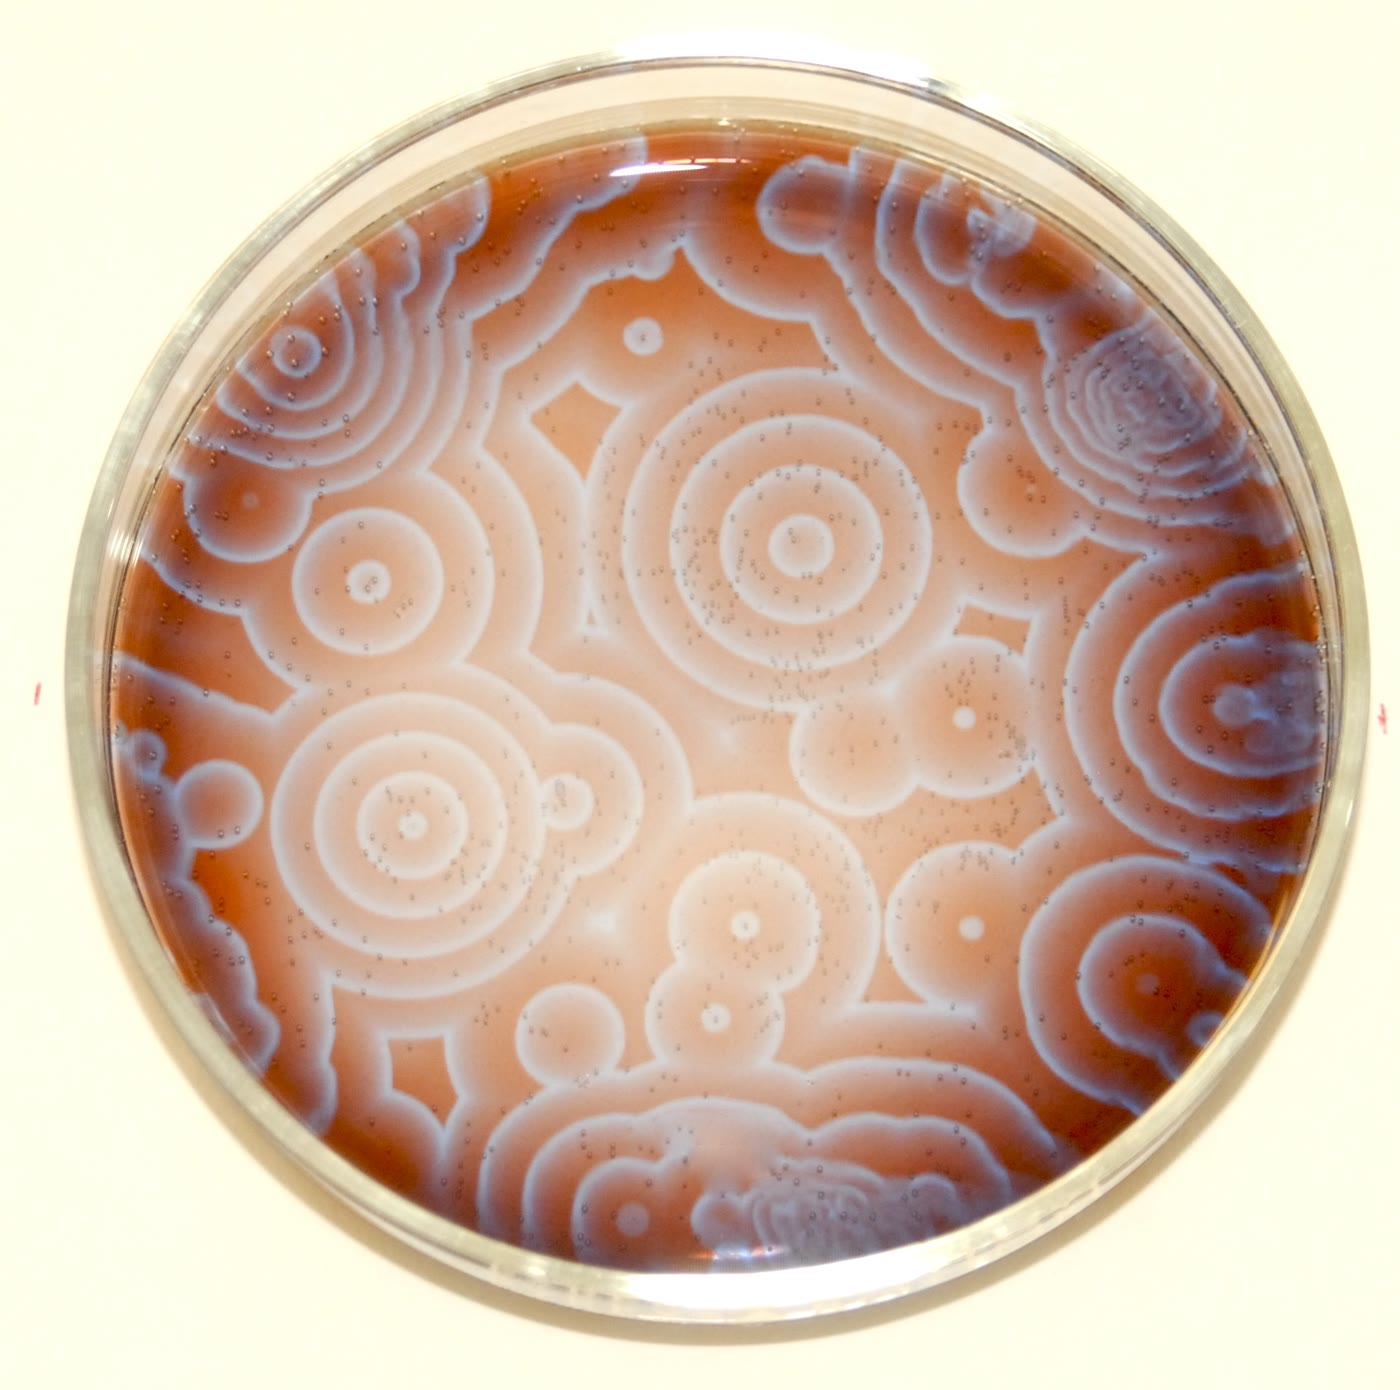
\includegraphics[width=0.48\linewidth]{images/book4/bz-reaction.jpg}

{\small विलयन की एक पतली परत में बेलौसोव--झाबोटिंस्की अभिक्रिया की सर्पिल तरंगें:
हर नीला अग्रभाग उत्प्रेरक के ऑक्सीकरण की एक तरंग है, जो
अपचयित (लाल) माध्यम में बढ़ती है और उस क्षेत्र में पुनः प्रवेश नहीं कर सकती जिसे उसने अभी
छोड़ा है।}
\end{omfigure}

\begin{definition}[विश्रांति विधि, रासायनिक विश्रांति काल]\label{def:b3:complex-kinetics:relaxation}
\emph{विश्रांति विधि}\index{विश्रांति विधि} साम्य पर स्थित किसी निकाय को
अचानक (ताप, दाब या विद्युत क्षेत्र की छलाँग से) विक्षुब्ध करती है
और नए साम्य पर उसकी वापसी का अनुसरण करती है। छोटे विक्षोभ के लिए
विचलन चरघातांकी रूप से क्षीण होता है, \emph{रासायनिक विश्रांति
काल}\index{रासायनिक विश्रांति काल} $\tau$ के साथ।
\end{definition}

\begin{proposition}[संगुणन का विश्रांति काल]\label{prop:b3:complex-kinetics:relaxation-time}
$\mathrm{A + B \rightleftharpoons C}$ ($k_1$, $k_{-1}$) के लिए, छोटे विक्षोभ के बाद,
\[
  \frac1\tau = k_1([\mathrm A]_e + [\mathrm B]_e) + k_{-1} .
\]
\end{proposition}

\begin{proof}
$[\mathrm C] = [\mathrm C]_e + x$, $[\mathrm A] = [\mathrm A]_e - x$, $[\mathrm B] = [\mathrm B]_e - x$ लिखिए। तब $\dot x =
k_1([\mathrm A]_e - x)([\mathrm B]_e - x) - k_{-1}([\mathrm C]_e + x)$; $x$ रहित पद साम्य पर निरस्त हो जाते हैं,
और $x^2$ छोड़ने पर: $\dot x = -[k_1([\mathrm A]_e + [\mathrm B]_e) + k_{-1}]x$।
\end{proof}

अनेक सांद्रताओं पर $\tau$ मापने से $1/\tau$ की एक रेखा मिलती है, $[\mathrm A]_e +
[\mathrm B]_e$ के विरुद्ध, जिसकी ढलान $k_1$ और अंतःखंड $k_{-1}$ है: दोनों स्थिरांक ऐसे
निकाय पर प्रयोगों से जो साम्य से कभी कुछ प्रतिशत से अधिक नहीं हटता। मैनफ़्रेड
आइगेन ने इसी प्रकार विलयन की सबसे तीव्र अभिक्रियाएँ मापीं, उनमें
\ce{H3O+} का \ce{OH-} द्वारा उदासीनीकरण भी।

\begin{omfigure}
\begin{tikzpicture}
\begin{axis}[width=0.62\linewidth, height=5.0cm, xmin=0, xmax=780, ymin=0, ymax=1.05,
  axis lines=left, xlabel={$t$ / \unit{\micro s}}, ylabel={$([\mathrm C] - [\mathrm C]_e)/([\mathrm C]_0 - [\mathrm C]_e)$},
  tick label style={font=\small}, label style={font=\small},
  legend style={font=\scriptsize, draw=none, at={(0.97,0.97)}, anchor=north east},
  legend cell align=left]
\addplot[omDef, very thick] table[x=t_us, y=dC] {figdata/out/bachelor-3-chemical-relaxation.dat};
\addplot[omThm, thick, dashed] table[x=t_us, y=exp] {figdata/out/bachelor-3-chemical-relaxation.dat};
\legend{पूर्ण दर समीकरण, {$\eu^{-t/\tau}$, $\tau = \qty{156}{\micro s}$}}
\draw[black!40, densely dotted] (axis cs:156,0) -- (axis cs:156,0.368) -- (axis cs:0,0.368);
\end{axis}
\end{tikzpicture}

{\small ताप-छलाँग के बाद $\mathrm{A + B \rightleftharpoons C}$ की विश्रांति, जिसने उसके
साम्य स्थिरांक को 5\,\% घटाया (मॉडल: $k_1 = \qty{1.0e8}{L.mol^{-1}.s^{-1}}$, $k_{-1} = \qty{1.0e3}{s^{-1}}$,
कुल मिलाकर A और B के \qty{1.0e-4}{mol/L}): पूर्ण दर समीकरण और
$1/\tau = k_1([\mathrm A]_e + [\mathrm B]_e) + k_{-1}$ वाला चरघातांकी संपाती हैं।}
\end{omfigure}

\begin{definition}[रुद्ध प्रवाह, कौंध प्रकाश-अपघटन]\label{def:b3:complex-kinetics:fast}
\emph{रुद्ध-प्रवाह विधि}\index{रुद्ध-प्रवाह विधि} दो अभिकारक
विलयनों को लगभग एक मिलीसेकंड में मिलाती है, उन्हें एक मिश्रक से होकर एक
प्रेक्षण सेल में धकेलकर, फिर प्रवाह रोककर अवशोषकता या
\omterm{def:b3:electronic-spectroscopy:luminescence}{प्रतिदीप्ति} अभिलिखित करती है। \emph{कौंध प्रकाश-अपघटन}\index{कौंध प्रकाश-अपघटन} एक छोटे तीव्र प्रकाश
स्पंद से कोई क्रियाशील स्पीशीज़ बनाता है और एक
दूसरे, विलंबित प्रकाश-पुंज से उसकी अभिक्रियाओं का अनुसरण करता है।
\end{definition}

\begin{omfigure}
\begin{tikzpicture}[font=\small, >=Stealth]
  % two drive syringes
  \foreach \y/\lab in {1.1/A, -0.1/B}{
    \draw[thick] (0,\y) rectangle (2.2,\y+0.6);
    \fill[omDef!25] (0.6,\y+0.05) rectangle (2.15,\y+0.55);
    \draw[thick] (0.6,\y) -- (0.6,\y+0.6);
    \draw[thick] (-0.6,\y+0.3) -- (0.6,\y+0.3);
    \node at (1.4,\y+0.3) {\lab};
    \draw[thick] (2.2,\y+0.3) -- (2.8,\y+0.3);}
  \draw[thick] (2.8,1.4) -- (3.2,0.8) (2.8,0.2) -- (3.2,0.8);
  \node[draw, thick, circle, minimum size=5mm, fill=white] (mx) at (3.4,0.8) {};
  \node[font=\scriptsize, anchor=north] at (3.4,0.5) {मिश्रक};
  \draw[thick] (mx.east) -- (4.4,0.8);
  \draw[thick, fill=omThm!15] (4.4,0.55) rectangle (5.4,1.05);
  \node[font=\scriptsize, anchor=north west, align=left] at (5.0,0.5) {प्रेक्षण\\ सेल};
  \draw[->, omThm, thick] (4.9,2.0) -- (4.9,1.1) node[pos=0, above, font=\scriptsize] {प्रकाश};
  \draw[->, omThm, thick] (4.9,0.5) -- (4.9,-0.4) node[below, font=\scriptsize] {संसूचक};
  \draw[thick] (5.4,0.8) -- (6.2,0.8);
  \draw[thick] (6.2,0.5) rectangle (7.6,1.1);
  \draw[thick] (7.0,0.5) -- (7.0,1.1);
  \draw[thick] (7.0,0.8) -- (7.9,0.8);
  \draw[thick] (7.9,0.4) -- (7.9,1.2);
  \node[font=\scriptsize, anchor=south] at (6.9,1.15) {रोधक सिरिंज};
  \draw[->, black!60] (-1.2,1.4) -- (-0.7,1.4) node[pos=0, left, font=\scriptsize] {चालक};
  \draw[->, black!60] (-1.2,0.2) -- (-0.7,0.2);
\end{tikzpicture}

{\small एक रुद्ध-प्रवाह उपकरण। चालक दो सिरिंजों को धकेलता है; विलयन
मिश्रक में मिलते हैं और लगभग एक मिलीसेकंड में प्रेक्षण सेल भर देते हैं;
रोधक सिरिंज का प्लंजर एक अवरोधक से टकराता है, प्रवाह रुक जाता है, और
संसूचक ताज़ा मिश्रित विलयन की अभिक्रिया अभिलिखित करता है।}
\end{omfigure}

\begin{omfigure}
\begin{tikzpicture}
\begin{axis}[width=0.62\linewidth, height=5.0cm, xmin=0, xmax=20, ymin=0, ymax=5.5,
  axis lines=left, xlabel={$t$ / ms}, ylabel={$[\mathrm P_1]$ / \unit{\micro M}},
  tick label style={font=\small}, label style={font=\small}]
\addplot[omDef, very thick] table[x=t_ms, y=P_uM] {figdata/out/bachelor-3-michaelis-menten-burst.dat};
\addplot[black!45, dashed, domain=0:20] {1.28 + 0.2*x};
\draw[->, black!60] (axis cs:4.5,0.7) -- (axis cs:0.25,1.24);
\node[font=\scriptsize, anchor=west] at (axis cs:4.5,0.7) {प्रस्फोट आयाम, \qty{1.28}{\micro M}};
\end{axis}
\end{tikzpicture}

{\small एक रुद्ध-प्रवाह प्रस्फोट अभिलेख (सप्ताहांत समस्या के आँकड़े): दो-चरणीय \omterm{def:b3:complex-kinetics:enzyme}{एंज़ाइम} का
पहला उत्पाद एक तीव्र प्रस्फोट में प्रकट होता है जिसके बाद एक सीधी
रेखा आती है; खंडित रेखा स्थायी अवस्था को $t = 0$ तक पीछे बहिर्वेशित करती है।}
\end{omfigure}

\begin{inthelab}[एक रुद्ध-प्रवाह मापन]
दोनों सिरिंजें एक ही बफ़र में \omterm{def:b3:complex-kinetics:enzyme}{एंज़ाइम} और क्रियाधार विलयनों से भरी जाती हैं,
तापस्थापित की जाती हैं, और अभिलिखित शॉटों से पहले सेल को धोने के लिए कई बार चलाई
जाती हैं; हर अभिलेख पाँच से दस शॉटों पर औसत किया जाता है। मृत काल,
अर्थात् प्रेक्षण आरंभ होने पर मिश्रण की आयु, एक बार ज्ञात दर वाली
अभिक्रिया से मापा जाता है।
\end{inthelab}

\begin{safety}{\ghs[0.8cm]{GHS05}\ghs[0.8cm]{GHS06}\ghs[0.8cm]{GHS09}}
% ledger: ghs4:Br2
ब्रोमीन: एक वाष्पशील, घना लाल-भूरा द्रव; साँस से लेने पर घातक, गंभीर
दाह उत्पन्न करता है, जलीय जीवों के लिए अत्यंत विषैला। केवल धूम-हुड में, दस्तानों
और चेहरे की सुरक्षा के साथ प्रयुक्त; छलकाव को अपचयित करने के लिए सोडियम थायोसल्फ़ेट का
विलयन पास रखा जाता है।
\end{safety}

\begin{history}[बोडेन्स्टाइन और बेलौसोव]
माक्स बोडेन्स्टाइन और सैमुएल लिंड ने 1906 में हाइड्रोजन--ब्रोमीन दर नियम
मापा; येन्स क्रिस्टियानसेन, कार्ल हर्ट्ज़फ़ेल्ड और माइकल पोलान्यी ने
1919 में इस अध्याय की शृंखला क्रियाविधि से उसकी व्याख्या की। मॉस्को के एक जैवरसायनज्ञ
बोरिस बेलौसोव ने लगभग 1951 में, किसी उपापचयी चक्र का रासायनिक मॉडल खोजते हुए,
अपनी \omterm{def:b3:complex-kinetics:oscillating}{दोलनी अभिक्रिया} पाई; उनकी पांडुलिपि अस्वीकार कर दी गई, और 1959 में केवल एक
छोटा सार प्रकाशित हुआ। अनातोल झाबोटिंस्की ने 1960 के दशक में अभिक्रिया को
अपनाया और उसकी व्याख्या की; पूर्ण क्रियाविधि 1970 के दशक के आरंभ में
ज्ञात की गई।
\end{history}

\section{अभ्यास}

\begin{exercise}[$\star$]\label{exo:b3:complex-kinetics:1}
शृंखला $\ce{Cl2 -> 2 Cl}$, $\ce{Cl + H2 -> HCl + H}$, $\ce{H + Cl2 -> HCl + Cl}$, $\ce{2 Cl -> Cl2}$ के लिए
हर चरण और \omterm{def:b3:complex-kinetics:chain}{शृंखला वाहकों} के नाम दीजिए, और समग्र अभिक्रिया लिखिए।
\end{exercise}

\begin{exercise}[$\star$]\label{exo:b3:complex-kinetics:2}
एक लिंडेमान निकाय के लिए $k_2 = \qty{1.0e7}{s^{-1}}$ और $k_{-1} = \qty{1.0e10}{L.mol^{-1}.s^{-1}}$ (अभ्यास के
आँकड़े)। $[\mathrm M]_{1/2}$ और \qty{750}{K} पर संगत दाब परिकलित कीजिए।
\end{exercise}

\begin{exercise}[$\star$]\label{exo:b3:complex-kinetics:3}
$v/V_{\max}$ व्यक्त कीजिए, $[\mathrm S] = K_M$, $3K_M$ और $9K_M$ पर। कौन-सी सांद्रता
$V_{\max}$ का 90\,\% देती है?
\end{exercise}

\begin{exercise}[$\star$]\label{exo:b3:complex-kinetics:4}
% ledger: enz:median.kcatKM, visc:H2O.25C
एक \omterm{def:b3:complex-kinetics:enzyme}{एंज़ाइम} के लिए $k_{\mathrm{cat}} = \qty{100}{s^{-1}}$ और $K_M = \qty{0.80}{mM}$। उसका \omterm{def:b3:complex-kinetics:michaelis}{विशिष्टता
स्थिरांक} परिकलित कीजिए और उसकी तुलना जल में विसरण सीमा, \qty{7.4e9}{L.mol^{-1}.s^{-1}},
और विशिष्ट $10^5$~\unit{L.mol^{-1}.s^{-1}} से कीजिए।
\end{exercise}

\begin{exercise}[$\star\star$]\label{exo:b3:complex-kinetics:5}
विघटन $\ce{CH3CHO -> CH4 + CO}$ के लिए यह क्रियाविधि प्रस्तावित है: $\ce{CH3CHO -> CH3 +
CHO}$ ($k_1$); $\ce{CH3 + CH3CHO -> CH4 + CH3CO}$ ($k_2$); $\ce{CH3CO -> CH3 + CO}$ ($k_3$);
$\ce{2 CH3 -> C2H6}$ ($k_4$)। दिखाइए कि मेथेन के निर्माण की दर
$k_2(k_1/2k_4)^{1/2}[\ce{CH3CHO}]^{3/2}$ है।
\end{exercise}

\begin{exercise}[$\star\star$]\label{exo:b3:complex-kinetics:6}
\ce{H2} और \ce{Br2} की समान सांद्रताओं से आरंभ करके, $k' = 0.10$ के साथ, आधा
ब्रोमीन खपने पर दर कितने गुना गिर चुकी है? इस गिरावट का कितना भाग
निरोधन के कारण है?
\end{exercise}

\begin{exercise}[$\star\star$]\label{exo:b3:complex-kinetics:7}
एक मॉडल हाइड्रोजन--ऑक्सीजन मिश्रण (अभ्यास के आँकड़े) में शाखन का
दर स्थिरांक $f = 1000\,p$ है, दीवार समापन का $6000/p$ और त्रि-पिंड समापन का
$10\,p^2$, सभी \unit{s^{-1}} में, जहाँ $p$, kPa में है। वह दाब परास ज्ञात कीजिए जिसमें मिश्रण
विस्फोटित होता है।
\end{exercise}

\begin{exercise}[$\star\star$]\label{exo:b3:complex-kinetics:8}
प्रारंभिक दरें $\qty{0.20}{\micro M.s^{-1}}$ हैं, $[\mathrm S] = \qty{0.50}{mM}$ पर, और $\qty{0.40}{\micro M.s^{-1}}$,
\qty{2.0}{mM} पर। $K_M$ और $V_{\max}$ ज्ञात कीजिए।
\end{exercise}

\begin{exercise}[$\star\star$]\label{exo:b3:complex-kinetics:9}
किसी संदमक के \qty{50}{\micro M} के साथ एक \omterm{def:b3:complex-kinetics:enzyme}{एंज़ाइम}
($K_M = \qty{0.80}{mM}$) की लाइनवीवर--बर्क रेखा असंदमित रेखा से $1/v$ अक्ष पर मिलती है और
$1/[\mathrm S]$ अक्ष को \qty{-0.417}{mM^{-1}} पर काटती है। संदमन का प्रकार पहचानिए और $K_i$ परिकलित कीजिए।
\end{exercise}

\begin{exercise}[$\star\star\star$]\label{exo:b3:complex-kinetics:10}
$\mathrm{A + X \to 2\,X}$ के लिए, $k = \qty{0.50}{L.mol^{-1}.s^{-1}}$, $a_0 = \qty{1.00}{mol/L}$ और $x_0 = \qty{0.010}{mol/L}$ के साथ,
वह समय परिकलित कीजिए जिस पर X की अंतिम मात्रा का आधा उपस्थित हो, और
\omterm{def:b3:complex-kinetics:michaelis}{अधिकतम दर} का समय।
\end{exercise}

\begin{exercise}[$\star\star\star$]\label{exo:b3:complex-kinetics:11}
$A = 1$ वाले ब्रसेलेटर के लिए स्थायी अवस्था पर जैकोबी आव्यूह के \omterm{def:b3:quantum-model-systems:operator}{अभिलक्षणिक मान}
$B = 1.5$ और $B = 2.5$ के लिए परिकलित कीजिए, और हर स्थिति में स्थायी
अवस्था के निकट व्यवहार का वर्णन कीजिए।
\end{exercise}

\begin{exercise}[$\star\star\star$]\label{exo:b3:complex-kinetics:12}
$\mathrm{A + B \rightleftharpoons C}$ के लिए, $k_1 = \qty{1.0e8}{L.mol^{-1}.s^{-1}}$ और $k_{-1} = \qty{1.0e3}{s^{-1}}$, तथा
$[\mathrm A]_e = [\mathrm B]_e = \qty{2.70e-5}{mol/L}$ के साथ, $\tau$ परिकलित कीजिए। केवल विश्रांति
मापनों से आप दोनों दर स्थिरांक कैसे प्राप्त करेंगे?
\end{exercise}

\section{समस्या: एक एंज़ाइम, एक संदमक और एक खुराक}

\begin{problem}[{सप्ताहांत समस्या --- एक एंज़ाइम, एक संदमक और एक खुराक:
न्यूनतम वर्ग से माइकेलिस--मेंटेन प्राचल, किसी
स्पर्धी संदमक का संदमन स्थिरांक, दी हुई खुराक पर बची सक्रियता, और एक रुद्ध-प्रवाह
प्रस्फोट}]
\label{pb:b3:complex-kinetics:1}
% ledger: enz:median.kcatKM
एक \omterm{def:b3:complex-kinetics:enzyme}{एंज़ाइम} (परखों में $[\mathrm E]_0 = \qty{5.0}{nM}$) अपने क्रियाधार का जल-अपघटन करता है; प्रारंभिक दरें
(समस्या के आँकड़े):
\begin{center}\small
\begin{tabular}{lccccccc}
\hline
$[\mathrm S]$ / mM & 0.10 & 0.20 & 0.40 & 0.80 & 1.60 & 3.20 & 6.40 \\
$v$ / \unit{\micro M.s^{-1}} & 0.0566 & 0.0981 & 0.169 & 0.247 & 0.340 & 0.397 & 0.447 \\ \hline
\end{tabular}
\end{center}
एक संदमक की उपस्थिति में उसी प्रकार के समंजन $V_{\max}$ अपरिवर्तित देते हैं और
आभासी $K_M$: 0.79, 1.47, 2.38 और \qty{4.02}{mM}, $[\mathrm I] = 0$, 20, 50 और
\qty{100}{\micro M} पर। $[\mathrm E]_0 = \qty{2.0}{\micro M}$ और संतृप्त क्रियाधार के साथ एक रुद्ध-प्रवाह प्रयोग
अनुभाग 5 के चित्र वाला प्रस्फोट अभिलेख देता है (\qty{1.28}{\micro M} का प्रस्फोट,
दर स्थिरांक \qty{625}{s^{-1}} के साथ, फिर \qty{200}{\micro M.s^{-1}})।

\medskip\noindent\textbf{भाग I --- $K_M$ और $V_{\max}$।}
\begin{enumerate}
  \item प्रारंभिक दरें क्यों प्रयुक्त की जाती हैं?
  \item लाइनवीवर--बर्क आलेख खींचिए; उसकी न्यूनतम-वर्ग रेखा $K_M =
        \qty{0.773}{mM}$ और $V_{\max} = \qty{0.491}{\micro M.s^{-1}}$ देती है। उस पर किन बिंदुओं का प्रभुत्व है?
  \item प्रत्यक्ष अरैखिक समंजन क्यों वरीय है?
  \item अरैखिक समंजन $K_M = 0.801 \pm \qty{0.023}{mM}$ और $V_{\max} = 0.502 \pm
        \qty{0.005}{\micro M.s^{-1}}$ देता है। क्या लाइनवीवर--बर्क मान इनसे संगत हैं?
  \item $k_{\mathrm{cat}}$ परिकलित कीजिए।
  \item \omterm{def:b3:complex-kinetics:michaelis}{विशिष्टता स्थिरांक} परिकलित कीजिए।
  \item इसकी तुलना विसरण सीमा और एक विशिष्ट \omterm{def:b3:complex-kinetics:enzyme}{एंज़ाइम} से कीजिए।
\end{enumerate}

\medskip\noindent\textbf{भाग II --- संदमक।}
\begin{enumerate}[resume]
  \item आँकड़े किस प्रकार का संदमन दिखाते हैं?
  \item $K_M^{\mathrm{app}}$ को $[\mathrm I]$ के फलन के रूप में लिखिए।
  \item $K_M^{\mathrm{app}}$ की $[\mathrm I]$ के विरुद्ध न्यूनतम-वर्ग रेखा का अंतःखंड \qty{0.799}{mM} और
        ढलान \qty{0.0321}{mM.\micro M^{-1}} है। $K_i$ निकालिए।
  \item उसकी मानक त्रुटि \qty{0.9}{\micro M} है। 95\,\% अंतराल दीजिए ($t = 4.30$,
        दो स्वातंत्र्य कोटियों के लिए)।
  \item $K_i$ क्या मापता है?
\end{enumerate}

\medskip\noindent\textbf{भाग III --- बची सक्रियता।}
\begin{enumerate}[resume]
  \item बची सक्रियता के अंश, $v_i/v_0$, को $[\mathrm S]$ और
        $[\mathrm I]$ के फलन के रूप में व्यक्त कीजिए।
  \item $[\mathrm S] = K_M$ और $[\mathrm I] = K_i$ पर इसका मान निकालिए।
  \item $[\mathrm S] = K_M$ और $[\mathrm I] = 10K_i$ पर।
  \item $[\mathrm S] = 10K_M$ और $[\mathrm I] = 10K_i$ पर। टिप्पणी कीजिए।
  \item दिखाइए कि $[\mathrm S] = K_M$ पर 90\,\% संदमन के लिए $[\mathrm I] = 18K_i$ चाहिए।
  \item समंजित $K_i$ से वह सांद्रता परिकलित कीजिए।
\end{enumerate}

\medskip\noindent\textbf{भाग IV --- प्रस्फोट।}
\begin{enumerate}[resume]
  \item \omterm{def:b3:complex-kinetics:enzyme}{एंज़ाइम} दो चरणों में कार्य करता है, $\mathrm{E + S \to E{-}acyl + P_1}$ ($k_2$) फिर $\mathrm{E{-}acyl \to E +
        P_2}$ ($k_3$)। $\mathrm P_1$ एक प्रस्फोट में क्यों प्रकट होता है?
  \item प्रस्फोट आयाम $[\mathrm E]_0\bigl(k_2/(k_2 + k_3)\bigr)^2$ है। $k_2/(k_2 + k_3)$ निकालिए।
  \item स्थायी ढलान से $k_{\mathrm{cat}}$ परिकलित कीजिए और भाग I से तुलना कीजिए।
  \item प्रस्फोट दर स्थिरांक $k_2 + k_3$ है। $k_2$ और $k_3$ निकालिए।
  \item जाँचिए कि $k_{\mathrm{cat}} = k_2k_3/(k_2 + k_3)$।
  \item परिणाम बताइए: वह संदमक सांद्रता जो
        $[\mathrm S] = K_M$ पर 90\,\% संदमन देती है।
\end{enumerate}
\end{problem}
